%%%%%%%%%%%%%%%%%%%%%%%%%%%%%%%%%%%%%%%%%%%%%%%%%%%%%%%%%%%%%%%%%%%%%%%%%%%
%% This file is part of the book
%%
%% Algorithmic Graph Theory
%% http://code.google.com/p/graph-theory-algorithms-book/
%%
%% Copyright (C) 2009, 2010, 2011 Minh Van Nguyen <nguyenminh2@gmail.com>
%% Copyright (C) 2010 Nathann Cohen <nathann.cohen@gmail.com>
%%
%% See the file COPYING for copying conditions.
%%%%%%%%%%%%%%%%%%%%%%%%%%%%%%%%%%%%%%%%%%%%%%%%%%%%%%%%%%%%%%%%%%%%%%%%%%%

\chapter{Random Graphs}
\label{chap:random_graphs}

A random\index{random graph} graph can be thought of as being a member
from a collection of graphs having some common properties. Recall that
Algorithm~\ref{alg:trees_forests:random_binary_tree} allows us to
generate a random binary tree having at least one vertex. Fix a
positive integer $n$ and let $\cT$ be a collection of all binary trees
on $n$ vertices. It can be infeasible to generate all members of
$\cT$, so for most purposes we are only interested in randomly
generating a member of $\cT$. A binary tree of order $n$ generated in
this manner is said to be a random\index{random graph} graph. For
example, Algorithm~\ref{alg:random_graphs:random_simple_graph}
presents a procedure to construct a random graph that is simple and
undirected; the procedure is adapted from pages~4--7 of
Lau~\cite{Lau2007}.

\begin{itemize}
\item See Bollob{\'a}s~\cite{Bollobas2001}.

\item See Gerke~et~al.~\cite{GerkeEtAl2008} for a random planar graph
  process.

\item See Fusy~\cite{Fusy2009} for a linear algorithm on uniform
  random sampling of planar graphs.

\item See Broutin~\cite{Broutin2007} on random trees.
\end{itemize}

\begin{algorithm}[!htbp]
\index{algorithm!random}
\index{simple graph!random}
%%%%%%%%%%%%%%%%%%%%%%%%%%%%%%%%%%%%%%%%%%%%%%%%%%%%%%%%%%%%%%%%%%%%%%%%%%%
%% This file is part of the book
%%
%% Algorithmic Graph Theory
%% http://code.google.com/p/graph-theory-algorithms-book/
%%
%% Copyright (C) 2009, 2010, 2011 Minh Van Nguyen <nguyenminh2@gmail.com>
%%
%% See the file COPYING for copying conditions.
%%%%%%%%%%%%%%%%%%%%%%%%%%%%%%%%%%%%%%%%%%%%%%%%%%%%%%%%%%%%%%%%%%%%%%%%%%%

\DontPrintSemicolon
\SetAlgoNoLine
%%
%% data section
\SetKwData{MyFalse}{False}
\SetKwData{MyMax}{max}
\SetKwData{MyTrue}{True}
%%
%% input
\KwIn{Positive integers $n$ and $m$ specifying the order and size,
  respectively, of the output graph.}
%%
%% output
\KwOut{A random simple undirected graph with $n$ vertices and $m$
  edges. If $m$ exceeds the size of $K_n$, then $K_n$ is returned.}
\BlankLine
%%
%% algorithm body
\If{$n = 1$}{
  \Return $K_1$\;
}
$\MyMax \assign n(n - 1) / 2$\;
\If{$m > \MyMax$}{
  \Return $K_n$\;
}
$G \assign$ null graph\;
$A \assign n \times n$ adjacency matrix with entries $a_{ij}$\;
$a_{ij} \assign \MyFalse$ for $0 \leq i,j < n$\;
$i \assign 0$\;
\While{$i < m$}{
  $u \assign$ draw uniformly at random from $\{0, 1, \dots, n-1\}$\;
  $v \assign$ draw uniformly at random from $\{0, 1, \dots, n-1\}$\;
  \If{$u = v$}{
    continue with next iteration of loop\;
  }
  \If{$u > v$}{
    swap values of $u$ and $v$\;
  }
  \If{$a_{uv} = \MyFalse$}{
    add edge $uv$ to $G$\;
    $a_{uv} \assign \MyTrue$\;
    $i \assign i + 1$\;
  }
}
\Return $G$\;

\caption{Random simple undirected graph.}
\label{alg:random_graphs:random_simple_graph}
\end{algorithm}

\begin{algorithm}[!htbp]
\index{algorithm!random}
\index{simple graph!random}
%%%%%%%%%%%%%%%%%%%%%%%%%%%%%%%%%%%%%%%%%%%%%%%%%%%%%%%%%%%%%%%%%%%%%%%%%%%
%% This file is part of the book
%%
%% Algorithmic Graph Theory
%% http://code.google.com/p/graph-theory-algorithms-book/
%%
%% Copyright (C) 2009--2011 Minh Van Nguyen <nguyenminh2@gmail.com>
%%
%% See the file COPYING for copying conditions.
%%%%%%%%%%%%%%%%%%%%%%%%%%%%%%%%%%%%%%%%%%%%%%%%%%%%%%%%%%%%%%%%%%%%%%%%%%%

\DontPrintSemicolon
\SetAlgoNoLine
%%
%% input
\KwIn{Positive integer $n$ and a probability $0 < p < 1$.}
%%
%% output
\KwOut{A random graph from $G(n,p)$.}
\BlankLine
%%
%% algorithm body
$G \assign \overline{K_n}$\;
$V \assign \{0, 1, \dots, n - 1\}$\;
$E \assign$ $\{2$-combinations of $V\}$\;
\For{\rm each $e \in E$}{
  $r \assign$ draw uniformly at random from interval $(0,1)$\;
  \If{$r < p$}{
    add edge $e$ to $G$\;
  }
}
\Return $G$\;

\caption{Generate a random graph in $G(n,p)$.}
\label{alg:random_graphs:generate_random_Gnp}
\end{algorithm}


%% This section considers two closely related common models of random
%% graphs: the binomial model and the Erd\H{o}s-R\'enyi model. Both
%% models are considered to be processes for generating undirected simple
%% graphs satisfying certain parameters.


%%%%%%%%%%%%%%%%%%%%%%%%%%%%%%%%%%%%%%%%%%%%%%%%%%%%%%%%%%%%%%%%%%%%%%%%%%%

\section{Binomial random graph model}

Fix a positive integer $n$, a probability $p$, and a vertex set
$V = \{0, 1, \dots, n - 1\}$. The
\emph{binomial}\index{random graph!binomial}~(or
\emph{Bernoulli})\index{random graph!Bernoulli} random graph model,
denoted $G(n,p)$ and introduced by Gilbert~\cite{Gilbert1959}, is
formally a probability\index{probability space} space over the set of
undirected simple graphs on $n$ vertices. If $G$ is any element of the
probability space $G(n,p)$ and $ij$ is any edge for distinct
$i,j \in V$, then $ij$ occurs as an edge of $G$ independently with
probability $p$. In symbols, for any distinct pair $i,j \in V$ we have
\[
\Pr[ij \in E(G)]
=
p
\]
where all such events are mutually independent. Equivalently the model
$G(n,p)$ considers the collection of all undirected simple graphs on
$n$ vertices, each such graph having at most $\binom{n}{2}$ edges, $m$
actual edges, and an associated probability
%%
\begin{equation}
\label{eqn:random_graphs:probability_of_chosen_graph_binomial_model}
p^m (1 - p)^{\binom{n}{2} - m}.
\end{equation}
%%
Notice the latter's resemblance to the
binomial\index{binomial distribution} distribution. By
$G \in G(n,p)$ we mean that $G$ is a random graph of the space
$G(n,p)$ and having probability
distribution $G(n,p)$.

To generate a random graph in $G(n,p)$, start with $G$ being a graph
on $n$ vertices but no edges. Consider each of the $\binom{n}{2}$
possible edges in some order and add it independently to $G$ with
probability $p$. See
Algorithm~\ref{alg:random_graphs:generate_random_Gnp} for pseudocode
of the procedure. The runtime of
Algorithm~\ref{alg:random_graphs:generate_random_Gnp} depends on an
efficient algorithm for generating all $2$-combinations of a set of
$n$ objects. We could adapt
Algorithm~\ref{alg:tree_data_structures:generate_all_r_combinations}
to our needs or search for a more efficient algorithm; see
problem~\ref{chap:random_graphs}.\ref{prob:random_graphs:quadratic_generate_random_Gnp}
for discussion of an algorithm to generate a graph in $G(n,p)$ in
quadratic
time. Figure~\ref{fig:random_graphs:binomial_random_graph_25_nodes}
illustrates some graphs from $G(25,p)$ with $p = i/6$ for
$i = 0, 1, \dots, 5$.

The expected number of edges of any $G \in G(n,p)$ is
\[
\alpha
=
\E[|E|]
=
p \cdot \binom{n}{2}
=
\frac{p \cdot n!} {2! (n - 2)!}
\]
and the expected total degree is
\[
\beta
=
\E[\#\deg]
=
2p \cdot \binom{n}{2}
=
pn(n - 1).
\]
Then the expected degree of each edge is $p(n - 1)$. From
problem~\ref{chap:introduction}.\ref{prob:introduction:number_simple_graphs}
we know that the number of undirected simple graphs on $n$ vertices is
given by
\[
2^{n(n-1) / 2}
\]
where~\eqref{eqn:random_graphs:probability_of_chosen_graph_binomial_model}
is the probability of any of these graphs being the output of the
above procedure. Let $\kappa(n,m)$ be the number of graphs from
$G(n,p)$ that are connected and have size $m$, and by $\Pr[G_\kappa]$
is meant the probability that $G \in G(n,p)$ is connected. Apply
expression~\eqref{eqn:random_graphs:probability_of_chosen_graph_binomial_model}
to see that
\[
\Pr[G_\kappa]
=
\sum_{i=n-1}^{\binom{n}{2}}
\kappa(n,i) \cdot p^i (1 - p)^{\binom{n}{2} - i}
\]
where $n - 1$ is the least number of edges of any undirected connected
graph on $n$ vertices, i.e. the size of any spanning tree of a
connected graph in $G(n,p)$. Similarly define $\Pr[\kappa_{i,j}]$ to
be the probability that two distinct vertices $i,j$ of
$G \in G(n,p)$ are connected. Gilbert~\cite{Gilbert1959} showed that
as $n \to \infty$, the probabilities $\Pr[G_\kappa]$ and
$\Pr[\kappa_{i,j}]$ approach
\[
\Pr[G_\kappa] \to 1 - n(1 - p)^{n-1}
\]
and
\[
\Pr[\kappa_{i,j}] \to 1 - 2(1 - p)^{n-1}.
\]

\begin{figure}[!htbp]
\centering
%%%%%%%%%%%%%%%%%%%%%%%%%%%%%%%%%%%%%%%%%%%%%%%%%%%%%%%%%%%%%%%%%%%%%%%%%%%
%% This file is part of the book
%%
%% Algorithmic Graph Theory
%% http://code.google.com/p/graph-theory-algorithms-book/
%%
%% Copyright (C) 2009, 2010, 2011 Minh Van Nguyen <nguyenminh2@gmail.com>
%%
%% See the file COPYING for copying conditions.
%%%%%%%%%%%%%%%%%%%%%%%%%%%%%%%%%%%%%%%%%%%%%%%%%%%%%%%%%%%%%%%%%%%%%%%%%%%

\documentclass{article}

\usepackage{subfigure}
\usepackage{tikz}
\usetikzlibrary{external}
\tikzexternalize{binomial-random-graphs-25-nodes}

\begin{document}

\begin{figure}
\subfigure[$p = 0$;
  $\alpha = 0$, $|E| = 0$;
  $\beta = 0$, $\#\deg = 0$]{
\begin{tikzpicture}
[lineDecorate/.style={-,thick},%
  nodeDecorate/.style={shape=circle,inner sep=2pt,draw,thick},
  scale=3.4]
%% nodes or vertices
\foreach \nodename/\x/\y in {
  0/1.00000000000000/0.000000000000000,
  1/0.968583161128631/0.248689887164855,
  2/0.876306680043864/0.481753674101715,
  3/0.728968627421412/0.684547105928689,
  4/0.535826794978997/0.844327925502015,
  5/0.309016994374947/0.951056516295154,
  6/0.0627905195293135/0.998026728428272,
  7/-0.187381314585725/0.982287250728689,
  8/-0.425779291565073/0.904827052466019,
  9/-0.637423989748690/0.770513242775789,
  10/-0.809016994374947/0.587785252292473,
  11/-0.929776485888251/0.368124552684678,
  12/-0.992114701314478/0.125333233564305,
  13/-0.992114701314478/-0.125333233564304,
  14/-0.929776485888251/-0.368124552684678,
  15/-0.809016994374947/-0.587785252292473,
  16/-0.637423989748690/-0.770513242775789,
  17/-0.425779291565072/-0.904827052466020,
  18/-0.187381314585725/-0.982287250728689,
  19/0.0627905195293128/-0.998026728428272,
  20/0.309016994374947/-0.951056516295154,
  21/0.535826794978996/-0.844327925502016,
  22/0.728968627421411/-0.684547105928689,
  23/0.876306680043864/-0.481753674101715,
  24/0.968583161128631/-0.248689887164855}
{
  \node (\nodename) at (\x,\y) [nodeDecorate] {};
}
\end{tikzpicture}
}
%%
%%
\qquad
\subfigure[$p = 1/6$;
  $\alpha = 50$, $|E| = 44$;
  $\beta = 100$, $\#\deg = 88$]{
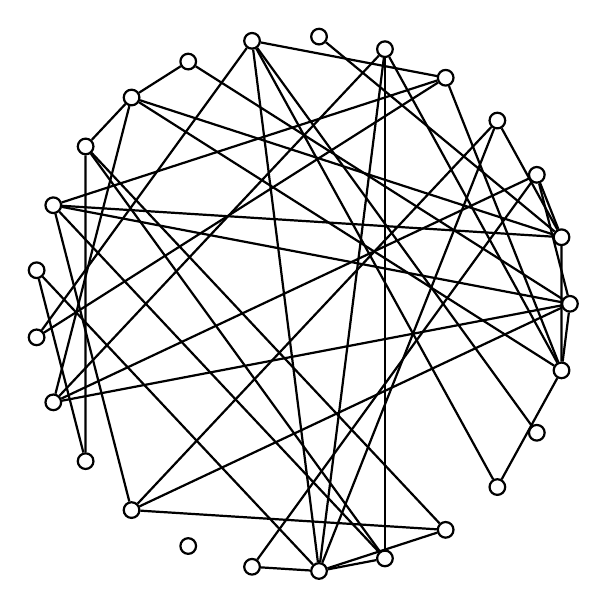
\begin{tikzpicture}
[lineDecorate/.style={-,thick},%
  nodeDecorate/.style={shape=circle,inner sep=2pt,draw,thick},
  scale=3.4]
%% nodes or vertices
\foreach \nodename/\x/\y in {
  0/1.00000000000000/0.000000000000000,
  1/0.968583161128631/0.248689887164855,
  2/0.876306680043864/0.481753674101715,
  3/0.728968627421412/0.684547105928689,
  4/0.535826794978997/0.844327925502015,
  5/0.309016994374947/0.951056516295154,
  6/0.0627905195293135/0.998026728428272,
  7/-0.187381314585725/0.982287250728689,
  8/-0.425779291565073/0.904827052466019,
  9/-0.637423989748690/0.770513242775789,
  10/-0.809016994374947/0.587785252292473,
  11/-0.929776485888251/0.368124552684678,
  12/-0.992114701314478/0.125333233564305,
  13/-0.992114701314478/-0.125333233564304,
  14/-0.929776485888251/-0.368124552684678,
  15/-0.809016994374947/-0.587785252292473,
  16/-0.637423989748690/-0.770513242775789,
  17/-0.425779291565072/-0.904827052466020,
  18/-0.187381314585725/-0.982287250728689,
  19/0.0627905195293128/-0.998026728428272,
  20/0.309016994374947/-0.951056516295154,
  21/0.535826794978996/-0.844327925502016,
  22/0.728968627421411/-0.684547105928689,
  23/0.876306680043864/-0.481753674101715,
  24/0.968583161128631/-0.248689887164855}
{
  \node (\nodename) at (\x,\y) [nodeDecorate] {};
}
%% edges or lines
\path
\foreach \startnode/\endnode in {
  0/2, 0/8, 0/11, 0/14, 0/16, 0/24, 1/2, 1/3, 1/6, 1/9, 1/11, 1/24,
  2/14, 2/18, 3/16, 3/19, 4/7, 4/11, 4/13, 4/24, 5/14, 5/19, 5/20, 5/24,
  7/13, 7/19, 7/22, 7/23, 8/9, 9/10, 9/14, 9/24, 10/15, 10/20, 10/21,
  11/16, 11/20, 12/15, 12/19, 16/21, 18/19, 19/20, 19/21, 22/24}
{
  (\startnode) edge[lineDecorate] node {} (\endnode)
};
\end{tikzpicture}
}
%%
%%
\subfigure[$p = 1/3$;
  $\alpha = 100$, $|E| = 108$;
  $\beta = 200$, $\#\deg = 212$]{
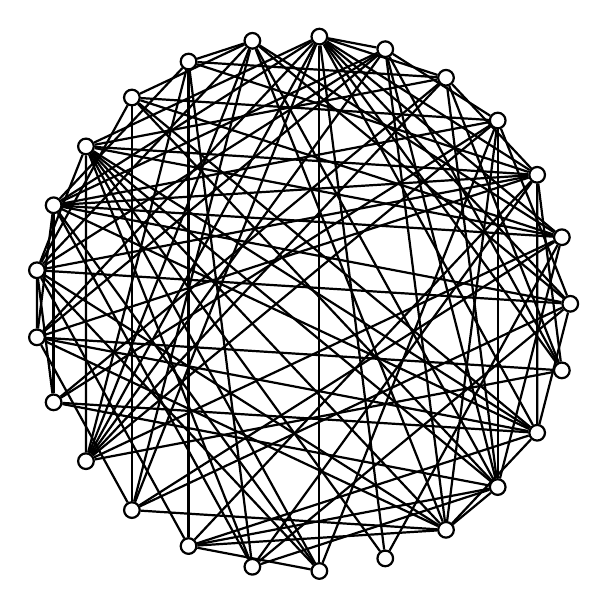
\begin{tikzpicture}
[lineDecorate/.style={-,thick},%
  nodeDecorate/.style={shape=circle,inner sep=2pt,draw,thick},
  scale=3.4]
%% nodes or vertices
\foreach \nodename/\x/\y in {
  0/1.00000000000000/0.000000000000000,
  1/0.968583161128631/0.248689887164855,
  2/0.876306680043864/0.481753674101715,
  3/0.728968627421412/0.684547105928689,
  4/0.535826794978997/0.844327925502015,
  5/0.309016994374947/0.951056516295154,
  6/0.0627905195293135/0.998026728428272,
  7/-0.187381314585725/0.982287250728689,
  8/-0.425779291565073/0.904827052466019,
  9/-0.637423989748690/0.770513242775789,
  10/-0.809016994374947/0.587785252292473,
  11/-0.929776485888251/0.368124552684678,
  12/-0.992114701314478/0.125333233564305,
  13/-0.992114701314478/-0.125333233564304,
  14/-0.929776485888251/-0.368124552684678,
  15/-0.809016994374947/-0.587785252292473,
  16/-0.637423989748690/-0.770513242775789,
  17/-0.425779291565072/-0.904827052466020,
  18/-0.187381314585725/-0.982287250728689,
  19/0.0627905195293128/-0.998026728428272,
  20/0.309016994374947/-0.951056516295154,
  21/0.535826794978996/-0.844327925502016,
  22/0.728968627421411/-0.684547105928689,
  23/0.876306680043864/-0.481753674101715,
  24/0.968583161128631/-0.248689887164855}
{
  \node (\nodename) at (\x,\y) [nodeDecorate] {};
}
%% edges or lines
\path
\foreach \startnode/\endnode in {
  0/3, 0/6, 0/7, 0/11, 0/12, 0/16, 0/18, 0/23, 1/6, 1/7, 1/9, 1/10,
  1/11, 1/15, 1/16, 1/20, 1/22, 2/4, 2/6, 2/8, 2/10, 2/11, 2/12, 2/13,
  2/17, 2/18, 2/23, 2/24, 3/5, 3/9, 3/11, 3/14, 3/15, 3/19, 3/21, 3/22,
  4/6, 4/8, 4/10, 4/14, 4/15, 4/22, 4/24, 5/6, 5/11, 5/12, 5/13, 5/15,
  5/21, 5/22, 5/24, 6/10, 6/11, 6/13, 6/15, 6/16, 6/19, 6/20, 6/23,
  6/24, 7/8, 7/9, 7/12, 7/15, 7/16, 7/21, 7/22, 8/11, 8/15, 8/17, 8/18,
  9/12, 9/16, 9/22, 9/23, 10/12, 10/15, 10/18, 10/19, 10/20, 10/21,
  10/22, 10/23, 11/13, 11/14, 11/18, 11/19, 11/23, 12/13, 12/14, 12/17,
  12/19, 12/21, 13/16, 13/21, 13/23, 13/24, 14/22, 14/23, 15/24, 16/21,
  17/19, 17/21, 17/22, 17/23, 18/22, 21/22, 21/23}
{
  (\startnode) edge[lineDecorate] node {} (\endnode)
};
\end{tikzpicture}
}
%%
%%
\qquad
\subfigure[$p = 1/2$;
  $\alpha = 150$, $|E| = 156$;
  $\beta = 300$, $\#\deg = 312$]{
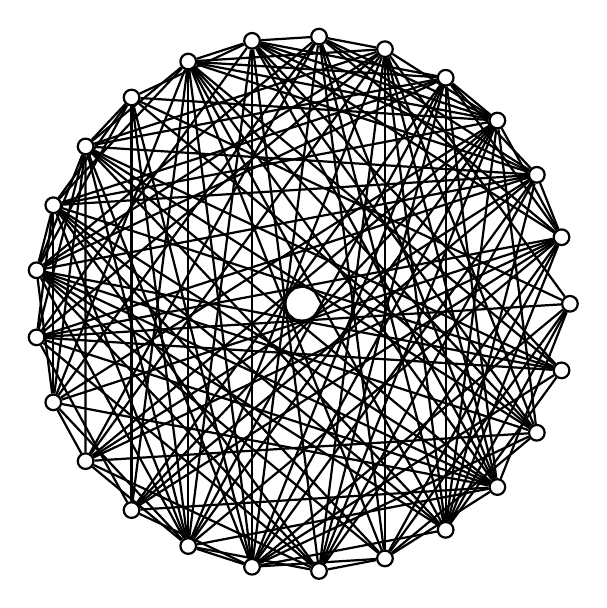
\begin{tikzpicture}
[lineDecorate/.style={-,thick},%
  nodeDecorate/.style={shape=circle,inner sep=2pt,draw,thick},
  scale=3.4]
%% nodes or vertices
\foreach \nodename/\x/\y in {
  0/1.00000000000000/0.000000000000000,
  1/0.968583161128631/0.248689887164855,
  2/0.876306680043864/0.481753674101715,
  3/0.728968627421412/0.684547105928689,
  4/0.535826794978997/0.844327925502015,
  5/0.309016994374947/0.951056516295154,
  6/0.0627905195293135/0.998026728428272,
  7/-0.187381314585725/0.982287250728689,
  8/-0.425779291565073/0.904827052466019,
  9/-0.637423989748690/0.770513242775789,
  10/-0.809016994374947/0.587785252292473,
  11/-0.929776485888251/0.368124552684678,
  12/-0.992114701314478/0.125333233564305,
  13/-0.992114701314478/-0.125333233564304,
  14/-0.929776485888251/-0.368124552684678,
  15/-0.809016994374947/-0.587785252292473,
  16/-0.637423989748690/-0.770513242775789,
  17/-0.425779291565072/-0.904827052466020,
  18/-0.187381314585725/-0.982287250728689,
  19/0.0627905195293128/-0.998026728428272,
  20/0.309016994374947/-0.951056516295154,
  21/0.535826794978996/-0.844327925502016,
  22/0.728968627421411/-0.684547105928689,
  23/0.876306680043864/-0.481753674101715,
  24/0.968583161128631/-0.248689887164855}
{
  \node (\nodename) at (\x,\y) [nodeDecorate] {};
}
%% edges or lines
\path
\foreach \startnode/\endnode in {
  0/5, 0/9, 0/13, 0/18, 0/20, 0/21, 0/22, 1/2, 1/3, 1/4, 1/6, 1/7, 1/13,
  1/14, 1/15, 1/16, 1/17, 1/19, 1/20, 1/21, 2/4, 2/6, 2/7, 2/8, 2/10,
  2/11, 2/12, 2/13, 2/15, 2/16, 2/18, 2/19, 2/21, 3/4, 3/5, 3/6, 3/7,
  3/8, 3/9, 3/11, 3/14, 3/15, 3/16, 3/17, 3/18, 3/19, 3/21, 3/23, 4/7,
  4/8, 4/10, 4/11, 4/12, 4/16, 4/17, 4/18, 4/19, 4/21, 4/22, 5/6, 5/8,
  5/10, 5/12, 5/13, 5/15, 5/17, 5/19, 5/20, 5/21, 5/22, 5/23, 6/7, 6/12,
  6/14, 6/15, 6/18, 6/20, 6/21, 6/22, 7/8, 7/9, 7/13, 7/17, 7/18, 7/19,
  7/22, 7/23, 7/24, 8/10, 8/11, 8/14, 8/16, 8/17, 8/18, 8/20, 8/21,
  8/22, 8/23, 8/24, 9/10, 9/11, 9/12, 9/16, 9/17, 9/18, 9/23, 10/12,
  10/13, 10/14, 10/15, 10/17, 10/18, 10/21, 10/22, 10/23, 10/24, 11/12,
  11/13, 11/14, 11/17, 11/19, 11/20, 11/21, 11/22, 11/24, 12/14, 12/17,
  12/19, 12/20, 12/21, 12/22, 12/23, 12/24, 13/16, 13/19, 13/22, 13/24,
  14/15, 14/17, 14/22, 15/17, 15/19, 15/23, 16/18, 16/22, 17/18, 17/19,
  17/22, 18/20, 18/21, 18/23, 18/24, 19/20, 20/22, 20/23, 21/24}
{
  (\startnode) edge[lineDecorate] node {} (\endnode)
};
\end{tikzpicture}
}
%%
%%
\subfigure[$p = 2/3$;
  $\alpha = 200$, $|E| = 185$;
  $\beta = 400$, $\#\deg = 370$]{
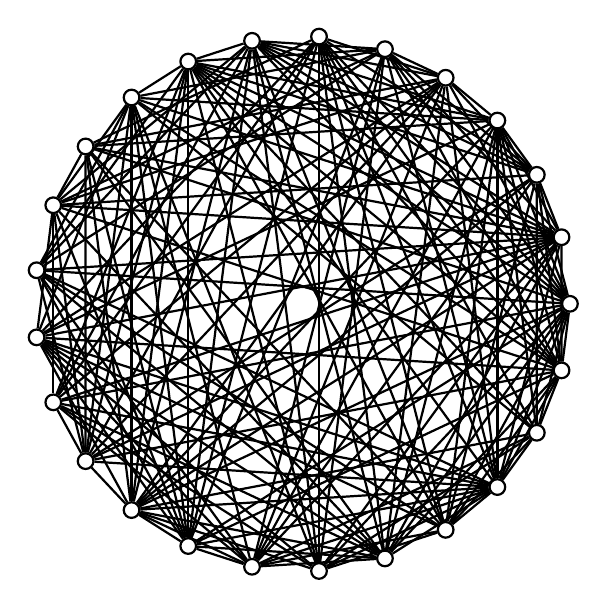
\begin{tikzpicture}
[lineDecorate/.style={-,thick},%
  nodeDecorate/.style={shape=circle,inner sep=2pt,draw,thick},
  scale=3.4]
%% nodes or vertices
\foreach \nodename/\x/\y in {
  0/1.00000000000000/0.000000000000000,
  1/0.968583161128631/0.248689887164855,
  2/0.876306680043864/0.481753674101715,
  3/0.728968627421412/0.684547105928689,
  4/0.535826794978997/0.844327925502015,
  5/0.309016994374947/0.951056516295154,
  6/0.0627905195293135/0.998026728428272,
  7/-0.187381314585725/0.982287250728689,
  8/-0.425779291565073/0.904827052466019,
  9/-0.637423989748690/0.770513242775789,
  10/-0.809016994374947/0.587785252292473,
  11/-0.929776485888251/0.368124552684678,
  12/-0.992114701314478/0.125333233564305,
  13/-0.992114701314478/-0.125333233564304,
  14/-0.929776485888251/-0.368124552684678,
  15/-0.809016994374947/-0.587785252292473,
  16/-0.637423989748690/-0.770513242775789,
  17/-0.425779291565072/-0.904827052466020,
  18/-0.187381314585725/-0.982287250728689,
  19/0.0627905195293128/-0.998026728428272,
  20/0.309016994374947/-0.951056516295154,
  21/0.535826794978996/-0.844327925502016,
  22/0.728968627421411/-0.684547105928689,
  23/0.876306680043864/-0.481753674101715,
  24/0.968583161128631/-0.248689887164855}
{
  \node (\nodename) at (\x,\y) [nodeDecorate] {};
}
%% edges or lines
\path
\foreach \startnode/\endnode in {
  0/2, 0/3, 0/4, 0/5, 0/6, 0/7, 0/8, 0/10, 0/12, 0/14, 0/16, 0/17, 0/19,
  0/20, 0/21, 0/22, 0/23, 0/24, 1/2, 1/3, 1/5, 1/7, 1/8, 1/9, 1/10,
  1/11, 1/12, 1/13, 1/14, 1/15, 1/16, 1/18, 1/19, 1/20, 1/22, 1/24, 2/3,
  2/4, 2/5, 2/6, 2/7, 2/8, 2/11, 2/15, 2/16, 2/18, 2/21, 2/23, 2/24,
  3/4, 3/7, 3/8, 3/9, 3/10, 3/13, 3/16, 3/18, 3/20, 3/21, 3/22, 3/23,
  3/24, 4/5, 4/6, 4/7, 4/10, 4/11, 4/13, 4/14, 4/15, 4/16, 4/18, 4/20,
  4/22, 5/7, 5/8, 5/9, 5/11, 5/12, 5/17, 5/18, 5/19, 5/22, 5/24, 6/10,
  6/13, 6/14, 6/15, 6/17, 6/19, 6/20, 6/21, 6/22, 6/23, 6/24, 7/8, 7/11,
  7/12, 7/14, 7/16, 7/17, 7/19, 7/20, 7/21, 7/24, 8/9, 8/12, 8/14, 8/15,
  8/16, 8/17, 8/19, 8/21, 8/22, 8/23, 8/24, 9/11, 9/12, 9/13, 9/15,
  9/16, 9/17, 9/18, 9/19, 9/23, 9/24, 10/11, 10/15, 10/16, 10/17, 10/20,
  10/21, 11/13, 11/14, 11/15, 11/17, 11/20, 11/24, 12/15, 12/17, 12/18,
  12/20, 12/21, 12/22, 13/16, 13/17, 13/18, 13/19, 13/20, 13/21, 13/22,
  13/24, 14/15, 14/18, 14/19, 14/20, 14/22, 15/16, 15/22, 15/24, 16/17,
  16/18, 16/19, 16/20, 16/22, 16/23, 17/18, 17/20, 17/22, 17/24, 18/20,
  18/21, 18/22, 18/23, 19/21, 19/22, 19/23, 20/22, 20/24, 21/22, 21/23,
  21/24, 22/23, 22/24, 23/24}
{
  (\startnode) edge[lineDecorate] node {} (\endnode)
};
\end{tikzpicture}
}
%%
%%
\qquad
\subfigure[$p = 5/6$;
  $\alpha = 250$, $|E| = 255$;
  $\beta = 500$, $\#\deg = 510$]{
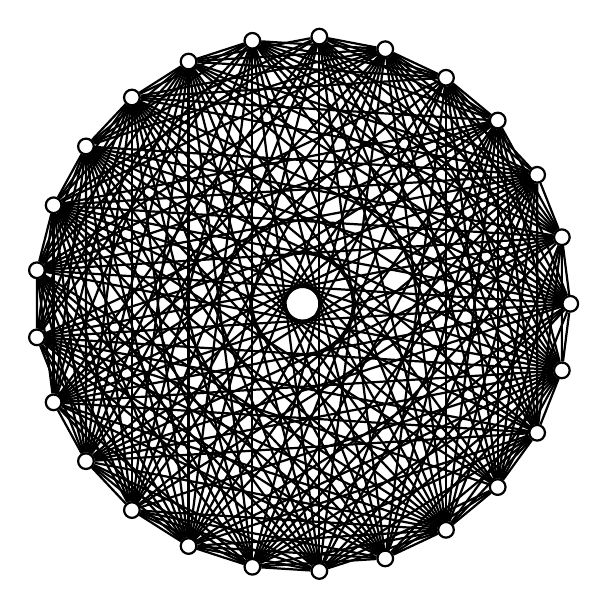
\begin{tikzpicture}
[lineDecorate/.style={-,thick},%
  nodeDecorate/.style={shape=circle,inner sep=2pt,draw,thick},
  scale=3.4]
%% nodes or vertices
\foreach \nodename/\x/\y in {
  0/1.00000000000000/0.000000000000000,
  1/0.968583161128631/0.248689887164855,
  2/0.876306680043864/0.481753674101715,
  3/0.728968627421412/0.684547105928689,
  4/0.535826794978997/0.844327925502015,
  5/0.309016994374947/0.951056516295154,
  6/0.0627905195293135/0.998026728428272,
  7/-0.187381314585725/0.982287250728689,
  8/-0.425779291565073/0.904827052466019,
  9/-0.637423989748690/0.770513242775789,
  10/-0.809016994374947/0.587785252292473,
  11/-0.929776485888251/0.368124552684678,
  12/-0.992114701314478/0.125333233564305,
  13/-0.992114701314478/-0.125333233564304,
  14/-0.929776485888251/-0.368124552684678,
  15/-0.809016994374947/-0.587785252292473,
  16/-0.637423989748690/-0.770513242775789,
  17/-0.425779291565072/-0.904827052466020,
  18/-0.187381314585725/-0.982287250728689,
  19/0.0627905195293128/-0.998026728428272,
  20/0.309016994374947/-0.951056516295154,
  21/0.535826794978996/-0.844327925502016,
  22/0.728968627421411/-0.684547105928689,
  23/0.876306680043864/-0.481753674101715,
  24/0.968583161128631/-0.248689887164855}
{
  \node (\nodename) at (\x,\y) [nodeDecorate] {};
}
%% edges or lines
\path
\foreach \startnode/\endnode in {
  0/1, 0/3, 0/4, 0/5, 0/6, 0/7, 0/8, 0/9, 0/10, 0/11, 0/12, 0/13, 0/14,
  0/15, 0/17, 0/18, 0/19, 0/22, 0/24, 1/2, 1/3, 1/4, 1/5, 1/6, 1/7, 1/8,
  1/10, 1/11, 1/12, 1/13, 1/14, 1/15, 1/16, 1/18, 1/21, 1/22, 1/23,
  1/24, 2/4, 2/5, 2/7, 2/8, 2/9, 2/10, 2/11, 2/12, 2/13, 2/14, 2/15,
  2/16, 2/17, 2/18, 2/19, 2/20, 2/21, 2/22, 2/23, 3/4, 3/5, 3/6, 3/7,
  3/9, 3/11, 3/12, 3/13, 3/14, 3/15, 3/17, 3/18, 3/19, 3/20, 3/21, 3/22,
  3/23, 3/24, 4/5, 4/6, 4/7, 4/8, 4/9, 4/12, 4/14, 4/16, 4/17, 4/18,
  4/20, 4/21, 4/22, 4/23, 4/24, 5/6, 5/7, 5/8, 5/9, 5/10, 5/11, 5/12,
  5/14, 5/15, 5/16, 5/17, 5/18, 5/19, 5/21, 5/22, 5/23, 5/24, 6/8, 6/10,
  6/11, 6/14, 6/15, 6/16, 6/17, 6/19, 6/20, 6/21, 6/22, 6/23, 6/24, 7/8,
  7/9, 7/10, 7/12, 7/13, 7/15, 7/16, 7/17, 7/18, 7/19, 7/20, 7/21, 7/23,
  7/24, 8/9, 8/10, 8/11, 8/12, 8/13, 8/14, 8/15, 8/16, 8/17, 8/18, 8/19,
  8/20, 8/21, 8/22, 8/24, 9/10, 9/11, 9/12, 9/13, 9/14, 9/15, 9/16,
  9/17, 9/18, 9/19, 9/20, 9/21, 9/22, 9/23, 9/24, 10/11, 10/12, 10/13,
  10/14, 10/15, 10/16, 10/17, 10/18, 10/19, 10/20, 10/21, 10/22, 10/23,
  10/24, 11/12, 11/13, 11/14, 11/15, 11/16, 11/17, 11/18, 11/19, 11/20,
  11/21, 11/22, 11/23, 11/24, 12/13, 12/14, 12/15, 12/16, 12/17, 12/18,
  12/19, 12/20, 12/21, 12/24, 13/15, 13/16, 13/17, 13/19, 13/20, 13/21,
  13/22, 13/23, 13/24, 14/15, 14/17, 14/18, 14/20, 14/21, 14/23, 14/24,
  15/16, 15/17, 15/18, 15/19, 15/21, 15/23, 15/24, 16/17, 16/18, 16/19,
  16/20, 16/21, 16/24, 17/18, 17/19, 17/20, 17/21, 17/23, 17/24, 18/19,
  18/20, 18/21, 18/23, 18/24, 19/21, 19/22, 19/23, 19/24, 20/21, 20/22,
  20/23, 20/24, 21/22, 21/23, 21/24, 22/23, 22/24, 23/24}
{
  (\startnode) edge[lineDecorate] node {} (\endnode)
};
\end{tikzpicture}
}
\end{figure}

\end{document}

\caption{Binomial random graphs $G(25,p)$ for various values of $p$.}
\label{fig:random_graphs:binomial_random_graph_25_nodes}
\end{figure}


%%%%%%%%%%%%%%%%%%%%%%%%%%%%%%%%%%%%%%%%%%%%%%%%%%%%%%%%%%%%%%%%%%%%%%%%%%%

\section{Erd\H{o}s-R\'enyi model}

Let $N$ be a fixed nonnegative integer. The
\emph{Erd\H{o}s-R\'enyi}~\cite{ErdosRenyi1960}
(or\index{random graph!Erd\H{o}s-R\'enyi}
\emph{uniform})\index{random graph!uniform} random graph model,
denoted $G(n,N)$, is a probability space over the set of undirected
graphs on $n$ vertices and exactly $N$ edges. Hence $G(n,N)$ can be
considered as a collection of $\binom{\binom{n}{2}} {N}$ undirected
graphs on exactly $N$ edges, each such graph being selected with equal
probability. To generate a graph in $G(n,N)$, start with $G$ being a
graph on $n$ vertices but no edges. Then choose $N$ of the possible
$\binom{n}{2}$ edges independently and uniformly at random and let
the chosen edges be the edge set of $G$. Each graph $G \in G(n,N)$ is
associated with a probability
\[
1 \left/ \binom{\binom{n}{2}} {N} \right..
\]

One of the first properties of random graphs which makes them so pleasant to work with is the following

\begin{theorem}
  Let $H$ be any graph, and $0<p<1$. Then
$$\lim_{n\to +\infty}P\left[H\text{ is an induced subgraph of }G_{n,p}\right]=1$$
\end{theorem}
\begin{proof}[Sketch]
Instinctively, we would like to find a copy of $H$ in $G_{n,p}$ by iteratively finding an acceptable representant $h(v_i)$ in $G_{n,p}$ of every vertex $v_i$ of $V(H) = \{v_1, \dots, v_k\}$. How could such a strategy work ?
\begin{itemize}
\item Pick for $v_1$ any vertex $h(v_1)\in G_{n,p}$
\item Pick for $v_2$ any vertex $h(v_2)\in G_{n,p}$ such that $h(v_1)h(v_2)\in E(G_{n,p})$ if $v_1v_2\in E(H)$, and such that $h(v_1)h(v_2)\not \in E(G_{n,p})$ otherwise
\item \dots
\item Assuming you have found, for all $i\leq j\leq k$, a representant $h(v_i)$ for each vertex $v_i$, and such that $H[\{v_1,\dots,v_{j-1}\}]$ is isomorphic to $G_{n,p}[\{h(v_1),\dots,h(v_{j-1})\}]$, try to find a new vertex $h(v_j)$ such that $\forall i<j,h(v_i)h(v_j)\in E(G_{n,p})$ if  and only if $v_iv_j\in E(H)$.

  When $n$ is growing large, such a vertex will exist with high probability.
\end{itemize}
\end{proof}

\begin{proof}
  Formally, let us write $H_i = H[\{v_1,\dots,v_{j-1}\}]$, and denote
  the probability that $H$ is an induced subgraph of $G_{n,p}$ by $P[H
    \mapsto_{ind} G_{n,p}]$. We can roughly bound the probability that $H_i$, but not $H_{i+1}$, is an induced subgraph of $G_{n,p}$ the following way :

  \begin{itemize}
  \item We put a copy of $H_i$ at any of the $\binom n i$ different $i$-subsets of $V(G_{n,p})$.

    This can be done, each time, in $i!$ different ways as the vertices $\{v_1, \dots, v_i\}$ can be permuted

  \item We compute the probability that no other vertex of $G_{n,p}$ can be used to complete our current copy of $H_i$ into a copy of $H_{i+1}$. The probability that such a vertex is acceptable being
    $$p^{d_{H_{i+1}}(v_{i+1})}(1-p)^{i-d_{H_{i+1}}(v_{i+1})}\geq min(p, 1-p)^i$$
    the property that none of the $n-i$ vertices left is acceptable is at most
    $$\left({ 1- min(p, 1-p)^i } \right)^{(n-i)}$$
  \end{itemize}

  As $0<p<1$, we can write $0<\epsilon = min(p, 1-p)$ and thus, the probability that $H_i$, but not $H_{i+1}$, is a induced subgraph of $G_{n,p}$ is at most $$i!\binom n i (1-\epsilon^i)^{n-i}\leq i! n^i (1-\epsilon^i)^{n-i} = o(1/n)$$
Which is asymptotically equal to 0 as $n$ grows.

Thus

\begin{align*}
  P[H \mapsto_{ind} G_{n,p}]&=1 - P[H_2 \mapsto_{ind} G_{n,p}, H_3\not \mapsto_{ind} G_{n,p}]\\
  &-P[H_3 \mapsto_{ind} G_{n,p}, H_4\not \mapsto_{ind} G_{n,p}]\\
  &\dots\\
  &-P[H_{k-1} \mapsto_{ind} G_{n,p}, H_k\not \mapsto_{ind} G_{n,p}]\\
  P[H \mapsto_{ind} G_{n,p}]&\geq 1-\sum_{i\leq k}i!n^i(1-\epsilon^i)^{n-i}\\
  &\geq 1-k\times o(1/n)\\
\end{align*}

Which proves the result.

\end{proof}

This proof also gives us a simple algorithm to find a copy of a graph $H$ into a random graph $G_{n,p}$. While obviously such an algorithm will not always find the copy of $H$ if it exists, the probability of a successful run will tend toward $1$ as proved immediately above.

\begin{lstlisting}
def find_induced(H, G):

    # f is the function from V(H) to V(G) we
    # are attempting to define
    f = {}

    # leftovers is the set of vertices of G which have not yet
    # been used by f
    G_leftovers = G.vertices()

    # Set of vertices for which no representant has been found yet
    H_leftovers = H.vertices()

    # While the function is not complete
    while H_leftovers:

        # We look for the next vertex of H
        v = H_leftovers.pop(0)

        # ... and look for its possible image
        candidates = [u for u in G_leftovers if
          all([ H.has_edge(h,v) == G.has_edge(f_h,u)
            for h,f_h in f.iteritems()])]

        if not candidates:
            raise ValueError("No copy of H has been found in G")

        # We pick the first of them
        f[v] = candidates[0]
        G_leftovers.remove(f[v])

    return f
\end{lstlisting}

Describe the random graph model of Erd\H{o}s and
R{\'e}nyi~\cite{ErdosRenyi1959}. Algorithms for efficient generation
of random networks; see Batagelj and
Brandes~\cite{BatageljBrandes2005}.


%%%%%%%%%%%%%%%%%%%%%%%%%%%%%%%%%%%%%%%%%%%%%%%%%%%%%%%%%%%%%%%%%%%%%%%%%%%

\section{Small-world networks}

The small-world network model of Watts and
Strogatz~\cite{WattsStrogatz1998}. The economic small-world model of
Latora and Marchiori~\cite{LatoraMarchiori2003}. See also
Milgram~\cite{Milgram1967}, Newman~\cite{Newman2003}, and Albert and
Barab{\'a}si~\cite{AlbertBarabasi2002}.


%%%%%%%%%%%%%%%%%%%%%%%%%%%%%%%%%%%%%%%%%%%%%%%%%%%%%%%%%%%%%%%%%%%%%%%%%%%

\section{Scale-free networks}

The power-law degree distribution model of Barab{\'a}si and
Albert~\cite{BarabasiAlbert1999}. See also Newman~\cite{Newman2003},
and Albert and Barab{\'a}si~\cite{AlbertBarabasi2002}.


%%%%%%%%%%%%%%%%%%%%%%%%%%%%%%%%%%%%%%%%%%%%%%%%%%%%%%%%%%%%%%%%%%%%%%%%%%%

\section{Evolving networks}

Preferential attachment models. See Newman~\cite{Newman2003},
and Albert and Barab{\'a}si~\cite{AlbertBarabasi2002}.


%%%%%%%%%%%%%%%%%%%%%%%%%%%%%%%%%%%%%%%%%%%%%%%%%%%%%%%%%%%%%%%%%%%%%%%%%%%

\section{Problems}

\begin{problem}
\item Modify Algorithm~\ref{alg:random_graphs:random_simple_graph} to
  generate the following random graphs.
  %%
  \begin{enumerate}[(a)]
  \item Simple weighted, undirected graph.

  \item Simple digraph.

  \item Simple weighted digraph.
  \end{enumerate}

\begin{algorithm}[!htbp]
\index{algorithm!random}
\index{simple graph!random}
%%%%%%%%%%%%%%%%%%%%%%%%%%%%%%%%%%%%%%%%%%%%%%%%%%%%%%%%%%%%%%%%%%%%%%%%%%%
%% This file is part of the book
%%
%% Algorithmic Graph Theory
%% http://code.google.com/p/graph-theory-algorithms-book/
%%
%% Copyright (C) 2009, 2010, 2011 Minh Van Nguyen <nguyenminh2@gmail.com>
%%
%% See the file COPYING for copying conditions.
%%%%%%%%%%%%%%%%%%%%%%%%%%%%%%%%%%%%%%%%%%%%%%%%%%%%%%%%%%%%%%%%%%%%%%%%%%%

\DontPrintSemicolon
\SetAlgoNoLine
%%
%% data section
\SetKwInOut{Input}{Input}
\SetKwInOut{Output}{Output}
%%
%% input/output
\Input{Positive integer $n$ and a probability $0 < p < 1$.}
\Output{A random graph from $G(n,p)$.}
\BlankLine
%%
%% algorithm body
$G \assign \overline{K_n}$\;
$V \assign \{1, 2, \dots, n\}$\;
\For{$i \assign 1, 2, \dots, n - 1$}{
  \For{$j \assign i + 1, i + 2, \dots, n$}{
    $r \assign$ draw uniformly at random from $[0,1)$\;
    \If{$r < p$}{
      add edge $ij$ to $G$\;
    }
  }
}
\Return $G$\;

\caption{Quadratic generation of a random graph in $G(n,p)$.}
\label{alg:random_graphs:quadratic_generate_random_Gnp}
\end{algorithm}

\item\label{prob:random_graphs:quadratic_generate_random_Gnp}
  Algorithm~\ref{alg:random_graphs:generate_random_Gnp} can be
  considered as a template for generating random graphs in
  $G(n,p)$. The procedure does not specify how to generate all the
  $2$-combinations of a set of $n > 1$ objects. Here we discuss how to
  construct all such $2$-combinations and derive a quadratic time
  algorithm for generating random graphs in $G(n,p)$.
  %%
  \begin{enumerate}[(a)]
  \item Consider a vertex set $V = \{0, 1, \dots, n - 1\}$ with at
    least two elements and let $E$ be the set of all $2$-combinations
    of $V$, where each $2$-combination is written $ij$. Show that
    $ij \in E$ if and only if $i < j$.

  \item From the previous exercise, we know that if $0 \leq i < n - 1$
    then there are $n - (i + 1)$ pairs $jk$ where either $i = j$ or
    $i = k$. Show that
    \[
    \sum_{i=0}^{n-2} (n - i - 1)
    =
    \frac{n^2 - n}{2}
    \]
    and conclude that
    Algorithm~\ref{alg:random_graphs:quadratic_generate_random_Gnp}
    has worst-case runtime $O((n^2 - n) / 2)$.
  \end{enumerate}
\end{problem}
